\newpage
\section{SYS\_10 - API Security}

\subsection{Introduzione alle API}

Un'Application Programming Interface (API) è un'interfaccia software che consente a differenti componenti applicative di comunicare tra loro in modo strutturato e standardizzato. Le API rappresentano uno dei pilastri fondamentali dei moderni sistemi distribuiti, poiché permettono l'integrazione tra servizi eterogenei, spesso sviluppati e gestiti in modo indipendente.

Un'API è definita formalmente da una \emph{API specification}, ovvero un documento o uno standard che descrive le modalità di interazione, i formati dei messaggi, le operazioni disponibili e i vincoli da rispettare. Un sistema che aderisce a tale specifica è detto \emph{provider} o \emph{espositore} dell'API, mentre il software che ne fa uso è il \emph{consumer}.

\subsection{Architetture e modelli di API}

\subsubsection{REST}

Il modello architetturale più diffuso per la progettazione di API è il paradigma REST (Representational State Transfer), introdotto da Roy Fielding nella sua tesi di dottorato nel 2000. REST non è un protocollo, ma uno stile architetturale per sistemi distribuiti basati su HTTP.

Le API REST adottano un'architettura client-server e sono intrinsecamente \emph{stateless}: ogni richiesta contiene tutte le informazioni necessarie per essere elaborata, senza che il server mantenga stato relativo al client tra una richiesta e l'altra. Questo approccio migliora la scalabilità e semplifica il bilanciamento del carico.

Un ulteriore principio chiave è l'interfaccia uniforme, che prevede l'identificazione delle risorse tramite URI e la loro manipolazione attraverso rappresentazioni, tipicamente in formato JSON o XML. Le operazioni sulle risorse sono mappate sui metodi HTTP standard, come GET, POST, PUT, DELETE e PATCH.

\begin{figure}[H]
    \centering
    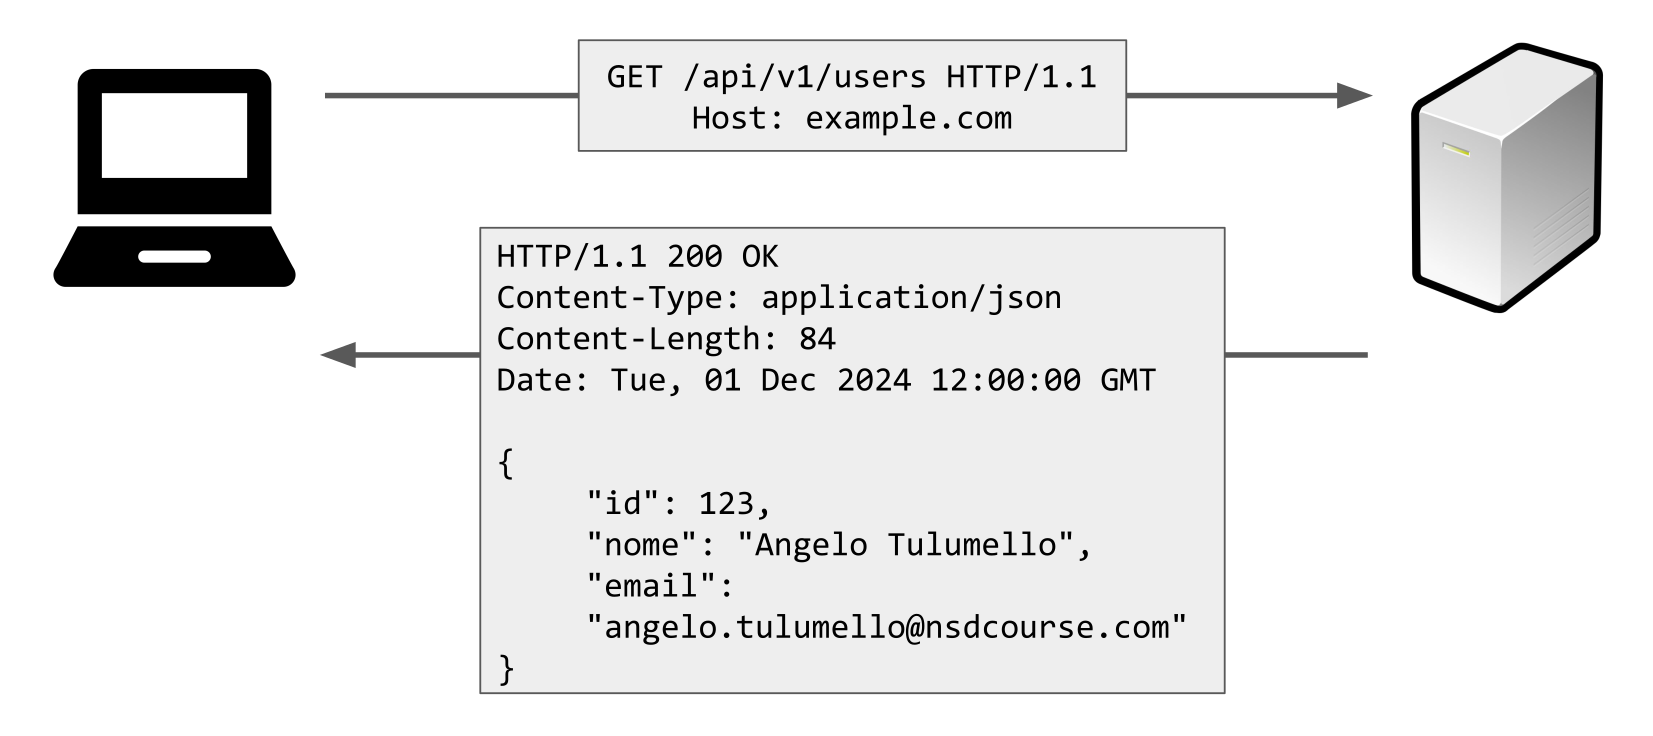
\includegraphics[width=.8\linewidth]{immagini/SYS_10/rest_api.png}
    \caption{Esempio di interazione tra client e server tramite API REST. Il client invia una richiesta HTTP GET all’endpoint \texttt{/api/v1/users} per ottenere la rappresentazione di una risorsa. Il server risponde con un messaggio HTTP \texttt{200 OK} contenente header informativi e il payload in formato JSON, che rappresenta lo stato corrente della risorsa richiesta.}
    \label{fig:rest_api}
\end{figure}



\subsubsection{Altri modelli di API}

Oltre a REST, esistono altri approcci rilevanti. SOAP è una tecnologia più datata, caratterizzata da un protocollo rigido e basato esclusivamente su XML, che incapsula le richieste all'interno di messaggi SOAP trasportati su HTTP.

GraphQL, introdotto da Facebook, è un linguaggio dichiarativo che consente al client di specificare esattamente quali dati desidera ottenere, riducendo fenomeni di over-fetching e under-fetching.

gRPC, sviluppato da Google, utilizza un protocollo binario ad alte prestazioni basato su HTTP/2 ed è particolarmente adatto a comunicazioni interne tra microservizi (east-west).

\subsection{Tipologie di API}

Le API possono essere classificate in base al tipo di consumatore. Le API Business-to-Consumer (B2C) sono tipicamente utilizzate da applicazioni web e mobile, mentre le API Business-to-Business (B2B) supportano l'integrazione tra organizzazioni, come nei sistemi di open banking o fatturazione elettronica.

Dal punto di vista dell'esposizione, si distingue tra API north-south, esposte verso l'esterno e quindi maggiormente soggette a minacce, e API east-west, utilizzate per la comunicazione interna tra servizi o dipartimenti.

\subsection{Concetto di API Security}

La sicurezza delle API è una branca della web application security che si occupa di proteggere le API da attacchi, abusi e violazioni. L'obiettivo è garantire che solo client autenticati e autorizzati possano accedere alle risorse, preservando confidenzialità, integrità e disponibilità dei dati.

L'importanza dell'API security è cresciuta in modo significativo con la diffusione di architetture a microservizi, applicazioni mobile e sistemi IoT, che fanno ampio affidamento sulle API come canale principale di comunicazione.

\subsection{API Security e Web Security tradizionale}

La sicurezza web tradizionale è storicamente fondata su un modello perimetrale, spesso descritto come \emph{“castle and moat”}. In questo paradigma, l’applicazione è protetta da un perimetro ben definito, all’interno del quale si assume che le entità siano affidabili, mentre l’accesso dall’esterno è rigidamente controllato tramite firewall, reverse proxy e Web Application Firewall (WAF). Questo approccio risulta efficace in contesti caratterizzati da un numero limitato di punti di ingresso e da protocolli relativamente statici.

\begin{figure}[H]
    \centering
    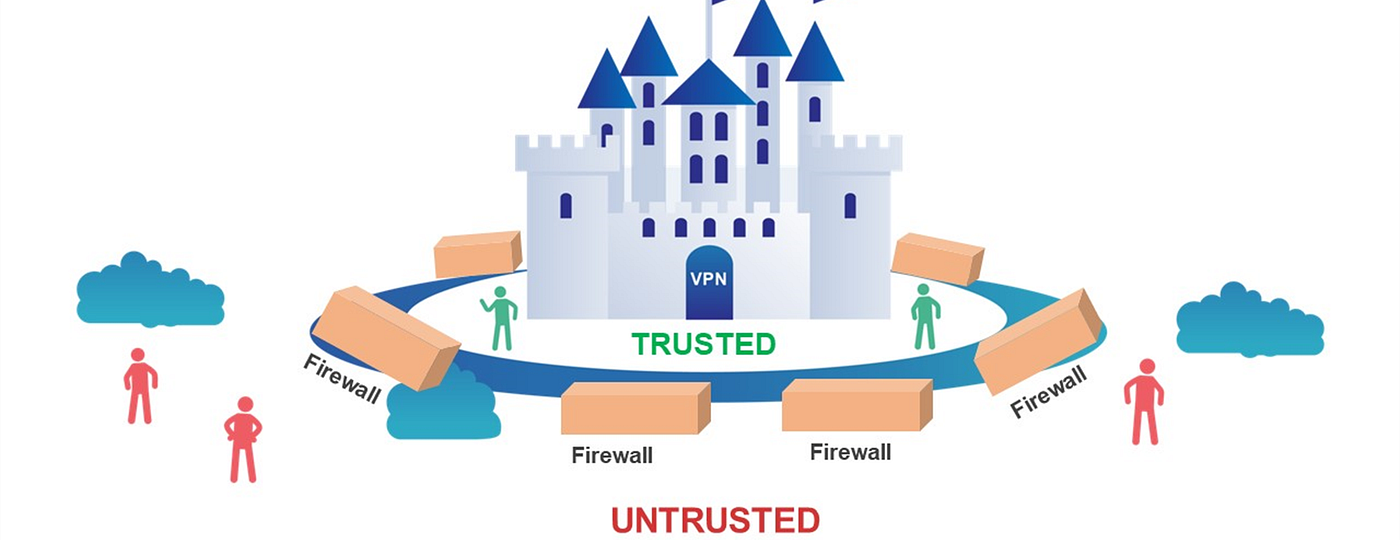
\includegraphics[width=.7\linewidth]{immagini/SYS_10/castle.png}
    \caption{Rappresentazione del modello di sicurezza perimetrale \emph{``castle and moat''}, in cui la fiducia è concentrata all’interno del perimetro di rete e l’accesso dall’esterno è filtrato tramite firewall e VPN.}

    \label{fig:castle}
\end{figure}


Le API moderne, invece, rompono questo modello. Esse espongono un numero elevato di endpoint, ciascuno potenzialmente accessibile in modo diretto, spesso senza passare attraverso interfacce web tradizionali. Le API sono progettate per essere consumate da applicazioni mobile, servizi backend, microservizi e sistemi automatizzati, piuttosto che da browser. Di conseguenza, molte delle assunzioni alla base della web security classica non risultano più valide.

Un primo limite riguarda l’uso dei Web Application Firewall. I WAF tradizionali sono ottimizzati per analizzare richieste HTTP generate da browser e per rilevare pattern noti di attacco, come Cross-Site Scripting o SQL Injection, basandosi su firme e regole statiche. Nel contesto delle API, tuttavia, il traffico è prevalentemente machine-to-machine, altamente strutturato e spesso legittimamente automatizzato. Questo rende complesso distinguere un uso corretto dell’API da un abuso malevolo, come data scraping o brute force logico, che non presenta necessariamente firme anomale evidenti.

Un’ulteriore differenza riguarda la stabilità dei formati di richiesta. Le applicazioni web tradizionali utilizzano protocolli e strutture di input relativamente stabili nel tempo. Al contrario, le API evolvono rapidamente, specialmente in ambienti DevOps e microservizi, dove nuove versioni, campi e parametri vengono introdotti frequentemente. Questa dinamicità rende difficile mantenere configurazioni di sicurezza statiche e richiede continui interventi di tuning manuale sui sistemi di protezione perimetrale.


\begin{figure}[H]
    \centering
    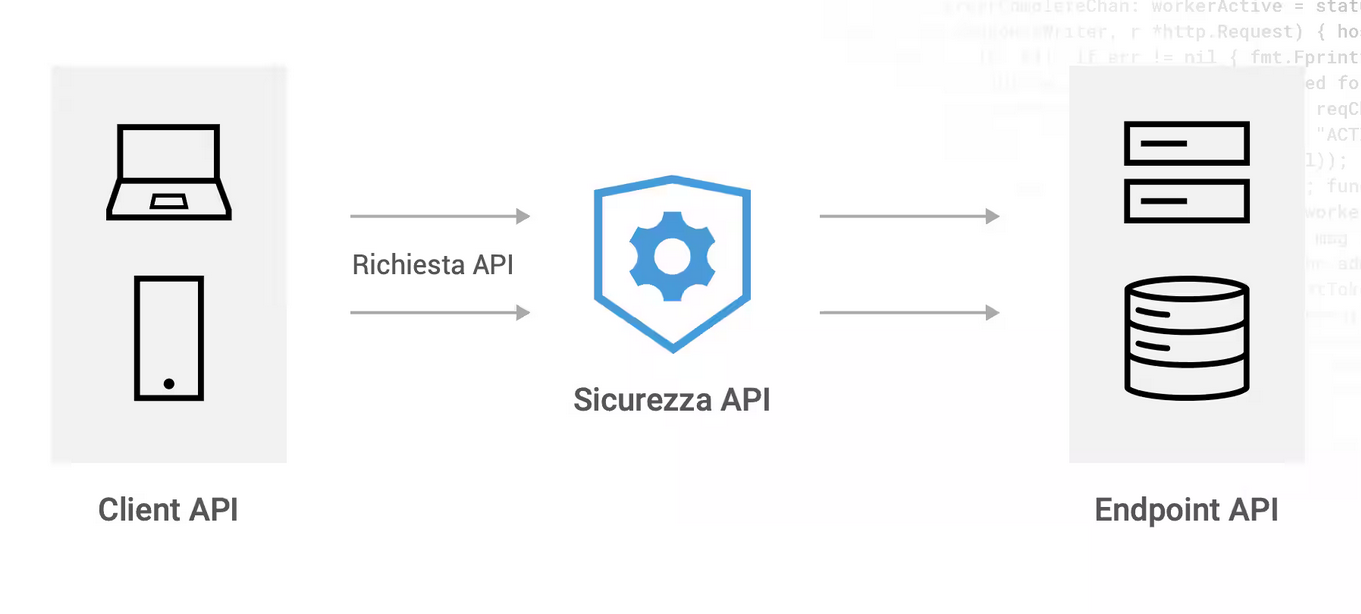
\includegraphics[width=.7\linewidth]{immagini/SYS_10/apisecurit}
    \caption{Schema concettuale della sicurezza delle API, che si interpone tra client e endpoint per controllare e proteggere le richieste di accesso alle risorse.}
    \label{fig:apisecutit}
\end{figure}


Inoltre, mentre nella web security classica l’identità dell’utente è spesso associata a una sessione browser, nelle API l’autenticazione è tipicamente basata su token, chiavi o credenziali applicative. Questo sposta il focus della sicurezza dall’analisi del contesto del client alla corretta implementazione di meccanismi di autenticazione, autorizzazione e validazione delle richieste a livello applicativo.

Alla luce di queste differenze, la sicurezza delle API non può essere affidata esclusivamente a controlli perimetrali. È necessario adottare un approccio \emph{security-by-design}, integrando i meccanismi di protezione direttamente nel ciclo di sviluppo del software. Ciò include la definizione rigorosa dei modelli di accesso, la validazione degli input, il controllo delle autorizzazioni a livello di risorsa e di operazione, nonché il monitoraggio continuo del comportamento delle API in produzione.

In sintesi, mentre la web security tradizionale protegge principalmente l’accesso a un’applicazione attraverso un perimetro ben definito, l’API security deve affrontare un ecosistema distribuito, dinamico e privo di confini netti, richiedendo strategie di difesa più granulari e adattive.

\subsection{Minacce comuni alle API}

Le API sono soggette a diverse classi di minacce, tra cui accessi non autorizzati dovuti a meccanismi di autenticazione deboli, attacchi di injection tramite input non validati, intercettazioni man-in-the-middle, denial of service e esposizione accidentale di dati sensibili, spesso causata da configurazioni errate come politiche CORS troppo permissive.

\\subsection{OWASP API Top 10}

L’Open Web Application Security Project (OWASP) pubblica periodicamente il documento \emph{OWASP API Security Top 10} con l’obiettivo di identificare e classificare le principali vulnerabilità che affliggono le API moderne. La lista non si limita a descrivere singoli bug di implementazione, ma mette in evidenza pattern ricorrenti di errori di progettazione, configurazione e controllo degli accessi, fornendo una visione sistematica dei rischi più comuni.

La vulnerabilità più critica, classificata come \texttt{API1:2023}, è la \emph{Broken Object Level Authorization} (BOLA). Il problema nasce dal fatto che molte API espongono endpoint che gestiscono oggetti identificabili tramite parametri controllabili dal client, come identificatori numerici o stringhe presenti negli URI. In assenza di controlli di autorizzazione a livello di singolo oggetto, un attaccante autenticato può manipolare tali identificatori per accedere a risorse appartenenti ad altri utenti. Un esempio reale è rappresentato da una vulnerabilità scoperta nel 2018 nell’API di Facebook Photos, che consentiva di accedere a immagini private semplicemente modificando l’identificatore della foto nell’endpoint. L’impatto è particolarmente elevato, poiché consente la lettura, la modifica o la cancellazione non autorizzata di dati sensibili. La mitigazione richiede l’implementazione sistematica di controlli di autorizzazione per ogni accesso a una risorsa, verificando che l’utente abbia effettivamente i privilegi necessari su quello specifico oggetto.

La \emph{Broken Authentication} (\texttt{API2:2023}) riguarda meccanismi di autenticazione deboli o implementati in modo errato. Il problema può derivare da una cattiva gestione dei token, da credenziali esposte o da flussi di autenticazione incompleti. Un caso emblematico è la vulnerabilità scoperta nel 2019 nelle API di Uber, che permetteva di accedere agli account di altri utenti riutilizzando un token valido e modificando l’identificatore dell’utente nelle richieste. L’impatto principale è l’impersonificazione degli utenti legittimi e l’accesso non autorizzato alle risorse protette. La mitigazione passa attraverso l’uso di protocolli di autenticazione robusti, una corretta gestione dei token di accesso e, ove possibile, l’adozione della multi-factor authentication.

La \emph{Broken Object Property Level Authorization} (\texttt{API3:2023}) si verifica quando l’API non applica controlli di accesso a livello delle singole proprietà di un oggetto. Il problema consente a un attaccante di leggere o modificare campi che dovrebbero essere protetti, spesso tramite tecniche di \emph{mass assignment}. Un esempio storico è rappresentato da una vulnerabilità riscontrata nel 2012 su GitHub, che consentiva agli utenti di assegnarsi privilegi amministrativi inviando campi non previsti all’interno delle richieste. L’impatto è l’esposizione o la manipolazione di informazioni sensibili. La mitigazione richiede l’adozione di allowlist esplicite per le proprietà accessibili e la validazione rigorosa dei dati forniti dal client.

L’\emph{Unrestricted Resource Consumption} (\texttt{API4:2023}) riguarda l’assenza di limiti sull’uso delle risorse, come CPU, memoria, banda o servizi esterni. Un caso significativo è l’attacco subito da GitHub nel 2018, in cui l’abuso delle API e l’assenza di adeguati limiti portarono a un attacco DDoS su larga scala basato su memcached. L’impatto include denial of service e costi operativi elevati. La mitigazione prevede l’introduzione di meccanismi di rate limiting, quote di utilizzo e limiti sulla dimensione delle richieste.

La \emph{Broken Function Level Authorization} (\texttt{API5:2023}) deriva da controlli inadeguati sull’accesso alle operazioni offerte dall’API. Un esempio tipico è rappresentato da sistemi di gestione dei contenuti in cui le API consentono operazioni di creazione o cancellazione di risorse senza verificare adeguatamente il ruolo dell’utente, permettendo così a utenti non amministrativi di eseguire funzioni riservate. L’impatto è l’esecuzione non autorizzata di azioni critiche. La mitigazione consiste nella definizione chiara dei ruoli e nella verifica dei privilegi prima dell’esecuzione di ogni funzione.

L’\emph{Unrestricted Access to Sensitive Business Flows} (\texttt{API6:2023}) riguarda l’esposizione di processi applicativi critici senza controlli contro l’automazione malevola. Un esempio reale è quello di piattaforme di e-commerce che permettevano l’applicazione illimitata di codici sconto tramite API, causando perdite economiche significative. La mitigazione include l’uso di controlli anti-automazione, limiti di frequenza e monitoraggio comportamentale.

La \emph{Server-Side Request Forgery} (\texttt{API7:2023}) si verifica quando un’API effettua richieste verso risorse esterne basandosi su input non validato. Nel 2022 diverse vulnerabilità SSRF sono state individuate nei servizi cloud di Microsoft Azure, consentendo agli attaccanti di accedere ai servizi di metadata interni e di ottenere token sensibili. La mitigazione richiede la validazione rigorosa degli endpoint di destinazione e l’uso di policy di rete restrittive.

La \emph{Security Misconfiguration} (\texttt{API8:2023}) comprende errori di configurazione dell’API o dei sistemi di supporto. Un caso noto è l’esposizione di migliaia di database MongoDB nel 2017, dovuta a configurazioni di default insicure che consentivano l’accesso non autenticato. La mitigazione prevede configurazioni sicure di default e revisioni periodiche.

L’\emph{Improper Inventory Management} (\texttt{API9:2023}) deriva dalla mancanza di un inventario aggiornato delle API esposte. Un esempio è la violazione subita da Panera Bread nel 2017, in cui un endpoint API non documentato ha esposto milioni di record di clienti. La mitigazione richiede una gestione strutturata del ciclo di vita delle API.

Infine, l’\emph{Unsafe Consumption of APIs} (\texttt{API10:2023}) riguarda la fiducia implicita nei servizi di terze parti. Un caso rilevante è una vulnerabilità nel login di Facebook del 2018, che permetteva di collegare account Instagram e Facebook senza adeguata verifica dell’identità, portando al takeover degli account. La mitigazione consiste nel trattare le API esterne come non fidate e validarne rigorosamente i dati.

\subsection{Best practice di prevenzione e protezione delle API}

La sicurezza delle API non può essere garantita esclusivamente tramite meccanismi di autenticazione e autorizzazione, ma richiede l’adozione di controlli preventivi in grado di limitare l’abuso delle funzionalità offerte e di proteggere l’infrastruttura applicativa. Le moderne best practice di API security mirano a ridurre la superficie di attacco e a garantire la resilienza dei servizi anche in presenza di traffico malevolo o anomalo.

Un primo elemento fondamentale è l’applicazione di meccanismi di \emph{rate limiting} e \emph{throttling}. Il rate limiting consente di limitare il numero massimo di richieste che un client può effettuare in un determinato intervallo di tempo, prevenendo attacchi di brute force, scraping e denial of service. Il throttling introduce invece una degradazione progressiva del servizio quando i limiti vengono avvicinati o superati, permettendo una gestione più controllata del carico. Questi meccanismi risultano essenziali per proteggere le API da un uso eccessivo anche quando le richieste sono formalmente valide e correttamente autenticate.

La mitigazione degli attacchi di tipo Distributed Denial of Service (DDoS) rappresenta un ulteriore aspetto critico. In questo contesto, l’uso di \emph{API Gateway} e \emph{Content Delivery Network} (CDN) consente di introdurre un punto di ingresso centralizzato per le richieste API, nel quale applicare controlli di sicurezza quali validazione degli input, autenticazione, rate limiting e caching. Le CDN e i servizi di protezione DDoS permettono inoltre di assorbire grandi volumi di traffico malevolo, migliorando la scalabilità e l’affidabilità del sistema e riducendo il carico sui servizi backend.

Un ruolo centrale è svolto anche dall’integrazione della sicurezza delle API nei processi di testing applicativo. Le best practice prevedono che la sicurezza venga verificata sistematicamente attraverso tecniche di \emph{Static Application Security Testing} (SAST), \emph{Dynamic Application Security Testing} (DAST) e test di penetrazione. L’integrazione di questi controlli nei pipeline di sviluppo consente di individuare vulnerabilità nelle API prima della messa in produzione, riducendo significativamente il rischio di esposizione.

\subsection{Best practice di rilevamento e monitoraggio delle API}

Oltre alle misure preventive, una strategia efficace di sicurezza delle API deve includere meccanismi di rilevamento e monitoraggio in grado di individuare comportamenti sospetti e attacchi che sfuggono ai controlli statici. In ambienti moderni e distribuiti, molte minacce si manifestano in modo graduale e richiedono un’osservazione continua del comportamento delle API.

La gestione efficace della sicurezza delle API richiede innanzitutto una conoscenza completa e aggiornata degli endpoint esposti. Il \emph{continuous API discovery} consente di mantenere un inventario costantemente aggiornato delle API, includendo endpoint interni, esterni e di terze parti. Questo approccio è fondamentale per individuare API non documentate o dimenticate, spesso definite come \emph{shadow APIs}, che possono rappresentare una superficie di attacco significativa.

Per affrontare le minacce note, è comune adottare meccanismi di \emph{signature-based threat detection}, che consentono di identificare pattern di attacco già conosciuti tramite l’uso di firme. Sebbene questa tecnica fornisca una protezione di base efficace, risulta limitata nel rilevare attacchi nuovi o comportamenti malevoli che non corrispondono a firme predefinite.

Per questo motivo, le architetture moderne di API security affiancano alle tecniche tradizionali strumenti di \emph{behavioral analytics} e \emph{intelligenza artificiale}. Analizzando i pattern di utilizzo delle API, questi sistemi sono in grado di identificare deviazioni rispetto al comportamento normale, consentendo il rilevamento di attacchi sofisticati e di tipo zero-day che si sviluppano gradualmente nel tempo.

Infine, la sicurezza delle API richiede attività di \emph{monitoring} e \emph{analysis} estese nel tempo. Il monitoraggio continuo delle API su più sessioni e periodi prolungati consente di individuare attacchi lenti e persistenti che potrebbero sfuggire a controlli di breve durata. La disponibilità dei dati di attività delle API è inoltre fondamentale per supportare analisi forensi, attività di incident response e la collaborazione tra team di sicurezza, sviluppo e operations.

\subsection{Meccanismi di autenticazione per le API}

L’autenticazione è un elemento critico per la sicurezza delle API, poiché garantisce che solo
utenti o sistemi autorizzati possano accedere alle risorse esposte. è fondamentale distinguere tra autenticazione, che verifica l’identità del chiamante, e autorizzazione, che determina quali operazioni tale soggetto è autorizzato a compiere. Una corretta implementazione dei meccanismi di autenticazione costituisce la base per prevenire accessi non autorizzati e abusi delle API.

\subsubsection{Basic Authentication}

La \emph{Basic Authentication} è uno dei meccanismi di autenticazione più semplici e storicamente diffusi. Essa utilizza una coppia di credenziali composta da username e password, che il client invia al server codificate in Base64 all’interno dell’header HTTP \texttt{Authorization}. Il server decodifica le credenziali e verifica l’identità del client prima di concedere o negare l’accesso.

Dal punto di vista dei vantaggi, la Basic Authentication è semplice da implementare ed è supportata nativamente dal protocollo HTTP. Tuttavia, presenta importanti limiti di sicurezza: le credenziali vengono inviate a ogni richiesta, la codifica Base64 non fornisce alcuna protezione crittografica e il meccanismo è sicuro solo se utilizzato esclusivamente su connessioni HTTPS. Per questi motivi, la Basic Authentication non è considerata adatta per API pubbliche o applicazioni mobile.

\subsubsection{API Keys}

Le \emph{API keys} rappresentano un meccanismo di autenticazione basato su un token statico assegnato a un client. La chiave può essere inviata come parametro della query o all’interno di un header HTTP dedicato. Il server verifica la validità della chiave prima di processare la richiesta.

Le API keys sono semplici da distribuire e consentono di tracciare l’utilizzo delle API e applicare politiche di rate limiting per client. Tuttavia, esse identificano l’applicazione chiamante piuttosto che l’utente finale e non forniscono meccanismi nativi di autorizzazione granulare. Inoltre, se intercettate, possono essere riutilizzate da un attaccante, rendendo necessaria una gestione attenta della rotazione e della revoca.

\subsubsection{Autenticazione basata su token}

I meccanismi di autenticazione basati su token rappresentano una soluzione più avanzata e flessibile. In questo modello, l’utente si autentica una sola volta fornendo le proprie credenziali e riceve un token di accesso, che viene poi utilizzato per le richieste successive. Il token viene inviato tipicamente tramite l’header HTTP \texttt{Authorization} con schema \texttt{Bearer}.

Questo approccio consente di implementare un’autenticazione stateless, migliorando la scalabilità delle API, poiché il server non è costretto a mantenere sessioni lato server. Tra i vantaggi principali figurano la flessibilità e la possibilità di includere nel token informazioni sull’identità e sui privilegi dell’utente. Tuttavia, i token possono risultare difficili da invalidare prima della loro scadenza e richiedono una gestione accurata per evitare abusi in caso di compromissione.

\subsubsection{JSON Web Token (JWT)}

I \emph{JSON Web Token} (JWT) sono uno standard aperto (RFC 7519) per la trasmissione sicura di informazioni tra due parti. Un JWT è composto da tre parti: \emph{header}, \emph{payload} e \emph{signature}. L’header specifica l’algoritmo di firma e il tipo di token, il payload contiene le \emph{claims}, ovvero le informazioni sull’utente o sul contesto di autenticazione, mentre la signature garantisce l’integrità del token.

Il flusso tipico prevede che l’utente si autentichi presso il server, il quale genera e restituisce un JWT. Il client invia quindi il token con ogni richiesta successiva, e il server verifica la validità della firma prima di concedere l’accesso. I JWT consentono un’autenticazione completamente stateless e sono particolarmente adatti ad architetture distribuite e microservizi.

Tra i principali vantaggi dei JWT figurano la scalabilità e la possibilità di includere direttamente nel token le informazioni necessarie per l’autorizzazione. Tuttavia, presentano anche alcune criticità: la revoca dei token è complessa, un token compromesso rimane valido fino alla scadenza e informazioni sensibili nel payload devono essere protette adeguatamente per evitare esposizioni.

Nel complesso, la scelta del meccanismo di autenticazione per le API dipende dal contesto applicativo, dai requisiti di sicurezza e dal tipo di client. In ambienti moderni, le soluzioni basate su token e JWT rappresentano lo standard de facto, mentre meccanismi più semplici come la Basic Authentication e le API keys sono limitati a scenari controllati o interni.


\subsection{OAuth 2.0 e OpenID Connect}

OAuth 2.0 è un framework di autorizzazione che consente a un'applicazione di accedere a risorse protette per conto di un utente, senza che quest'ultimo debba condividere le proprie credenziali. Il flusso più sicuro e diffuso è l'Authorization Code Flow, che separa l'autenticazione dall'accesso alle risorse.

OpenID Connect estende OAuth 2.0 introducendo un livello di autenticazione, tramite l'emissione di un ID Token che contiene informazioni sull'identità dell'utente, consentendo funzionalità come il Single Sign-On.


\begin{figure}[H]
    \centering
    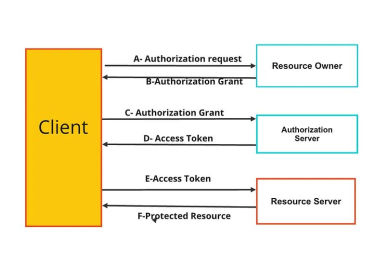
\includegraphics[width=.8\linewidth]{immagini/SYS_10/oauth}
    \caption{Flusso di autorizzazione OAuth~2.0 (Authorization Code Flow), che illustra l’interazione tra client, resource owner, authorization server e resource server per l’ottenimento e l’utilizzo di un access token.}
    \label{fig:oauth}
\end{figure}

\subsection{OpenID Connect}

OpenID Connect è un livello di identità (\emph{identity layer}) costruito sopra OAuth~2.0, con l’obiettivo di aggiungere funzionalità di autenticazione a un framework originariamente pensato per la delega dell’autorizzazione. Mentre OAuth~2.0 consente a un client di accedere a risorse protette per conto di un utente, OpenID Connect permette anche di verificare in modo standardizzato l’identità dell’utente stesso.

La principale estensione introdotta da OpenID Connect è l’emissione di un \emph{ID Token}, tipicamente sotto forma di JSON Web Token (JWT), che contiene informazioni sull’identità dell’utente autenticato. Questo meccanismo consente l’implementazione di funzionalità di \emph{Single Sign-On} (SSO), permettendo a un utente di autenticarsi una sola volta e accedere a più servizi.

Il flusso di OpenID Connect è simile all’Authorization Code Flow di OAuth~2.0, con la differenza che, oltre all’access token, viene rilasciato anche l’ID Token, utilizzato dal client per verificare l’identità dell’utente.

\begin{figure}[H]
    \centering
    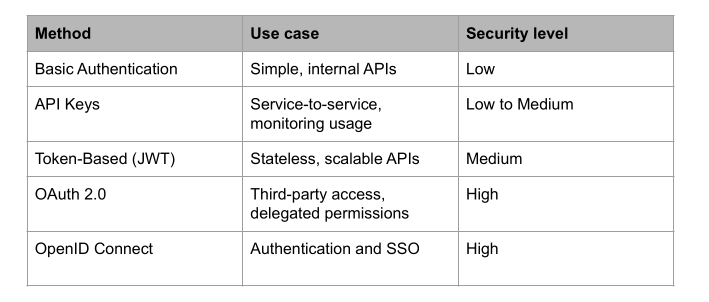
\includegraphics[width=.8\linewidth]{immagini/SYS_10/tabellaoa}
    \caption{Confronto tra i principali meccanismi di autenticazione utilizzati nelle API in termini di casi d’uso e livello di sicurezza.}
    \label{fig:tabelloa}
\end{figure}



\subsection{Best practice per la sicurezza delle API}

Una strategia efficace di API security richiede l'integrazione della sicurezza nel ciclo di vita del software, l'automazione dei controlli nei pipeline CI/CD, l'adozione di autenticazione forte e il rispetto del principio del minimo privilegio. È inoltre fondamentale implementare rate limiting, monitoraggio continuo, logging dettagliato e validazione rigorosa degli input.

La sicurezza delle API non è un'attività una tantum, ma un processo continuo che deve adattarsi all'evoluzione dell'ecosistema applicativo e delle minacce.
